\documentclass[11pt,letterpaper]{article}
\usepackage[utf8]{inputenc}

%----- Configuración del estilo del documento------%
\usepackage{epsfig,graphicx}
\usepackage[left=2cm,right=2cm,top=1.8cm,bottom=2.3cm]{geometry}
\usepackage{fancyhdr}
\usepackage{lastpage}
\usepackage{url}
\usepackage{tikz}
\pagestyle{fancy}
\fancyhf{}
\fancyhead[R]{\ifnum\value{page}>1 \textbf{Series de tiempo}\fi}
\rfoot{\textit{Página \thepage}}
%Encabezado izquierdo: logo
\lfoot{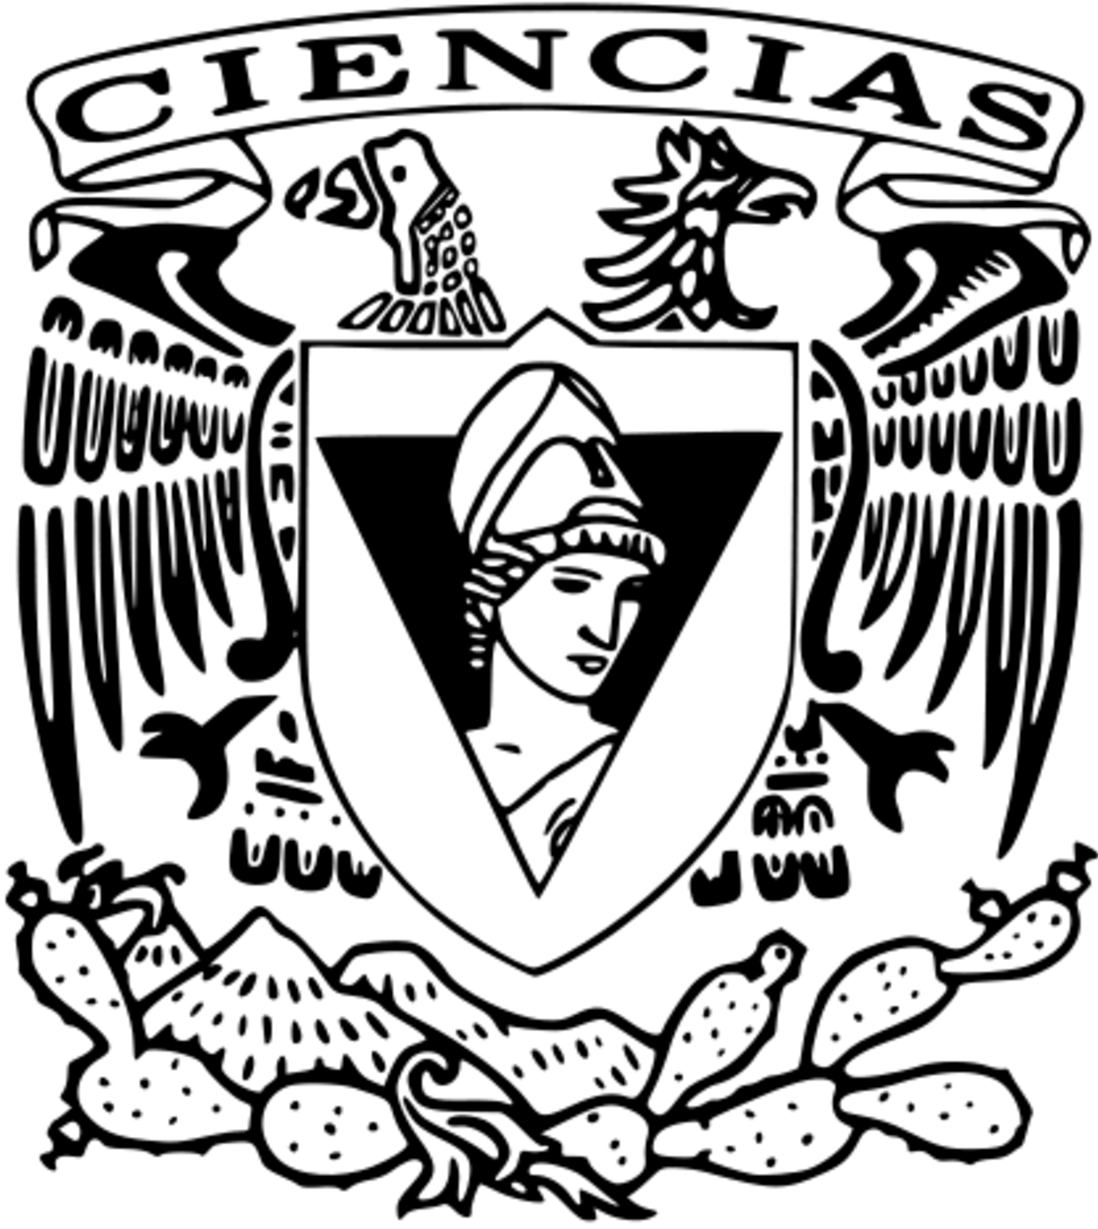
\includegraphics[height=1.0cm]{Logo_FC.png}}
%------ Paquetes matemáticos básicos --------%
\usepackage{amsmath}
\usepackage{amssymb}
\usepackage{amsthm}

\usepackage[spanish]{babel}
\usepackage{graphicx}
\usepackage{hyperref}

\usepackage{tabularx}
\usepackage{xcolor}
\usepackage[table]{xcolor}
\usepackage{colortbl}
\usepackage{array, multirow, multicol, tabularx}
\usepackage{tcolorbox}
\newtheorem{theorem}{Theorem}[section]
\newtheorem{corollary}{Corollary}[theorem]
\newtheorem{lemma}[theorem]{Lemma}

%------si-------%
\definecolor{B}{HTML}{FFFFFF}
\definecolor{G}{HTML}{5e5e5e}
\definecolor{R2}{HTML}{d53d40}
\definecolor{A2}{HTML}{034190}
\definecolor{V2}{HTML}{7faa50}
\newcommand{\R}{\mathbb{R}}
\newcommand{\C}{\mathcal{C}}
\newcommand{\N}{\mathbb{N}}
\newcommand{\Z}{\mathbb{Z}}
\newcommand{\Q}{\mathbb{Q}}
\renewcommand{\theenumi}{\Roman{enumi}}
\renewcommand{\labelenumi}{{\theenumi}.}

\begin{document}
%---Evironment--%
	\makeatletter
        \renewenvironment{proof}[1][\proofname]{\par
            \pushQED{\qed}%
            \normalfont \topsep6\p@\@plus6\p@\relax
            \trivlist
            \item\relax
            {\itshape
            #1\@addpunct{.}}\par\vspace{\baselineskip}\ignorespaces
            }{%
            \popQED\endtrivlist\@endpefalse
            }
        \newenvironment{Solucion}[1][Soluci\'on]{\par
            \pushQED{\qed}%
            \normalfont \topsep6\p@\@plus6\p@\relax
            \trivlist
            \item\relax
            {\itshape
            #1\@addpunct{.}}\par\vspace{\baselineskip}\ignorespaces
            }{%
            \popQED\endtrivlist\@endpefalse
            }
            
    \makeatother

%------ Encabezado -------- %

\begin{center}
    \begin{minipage}{3cm}
    	\begin{center}
    		\includegraphics[height=3.4cm]{logo_unam.png}
    	\end{center}
    \end{minipage}\hfill
    \begin{minipage}{10cm}
    	\begin{center}
    	\textbf{\large Universidad Nacional Autónoma de México}\\[0.1cm]
        \textbf{Facultad de Ciencias}\\[0.1cm]
        \textbf{\'Series de tiempo y modelos de supervivencia}\\[0.1cm]
        Tarea 1\\[0.1cm]
         El\'ias L\'opez Rivera\\[0.1cm]
        \texttt{ elias.lopezr,@ciencias.unam.mx }\\[0.1cm]
        Fecha:\,\,06/10/2026
    	\end{center}
    \end{minipage}\hfill
    \begin{minipage}{3cm}
    	\begin{center}
    		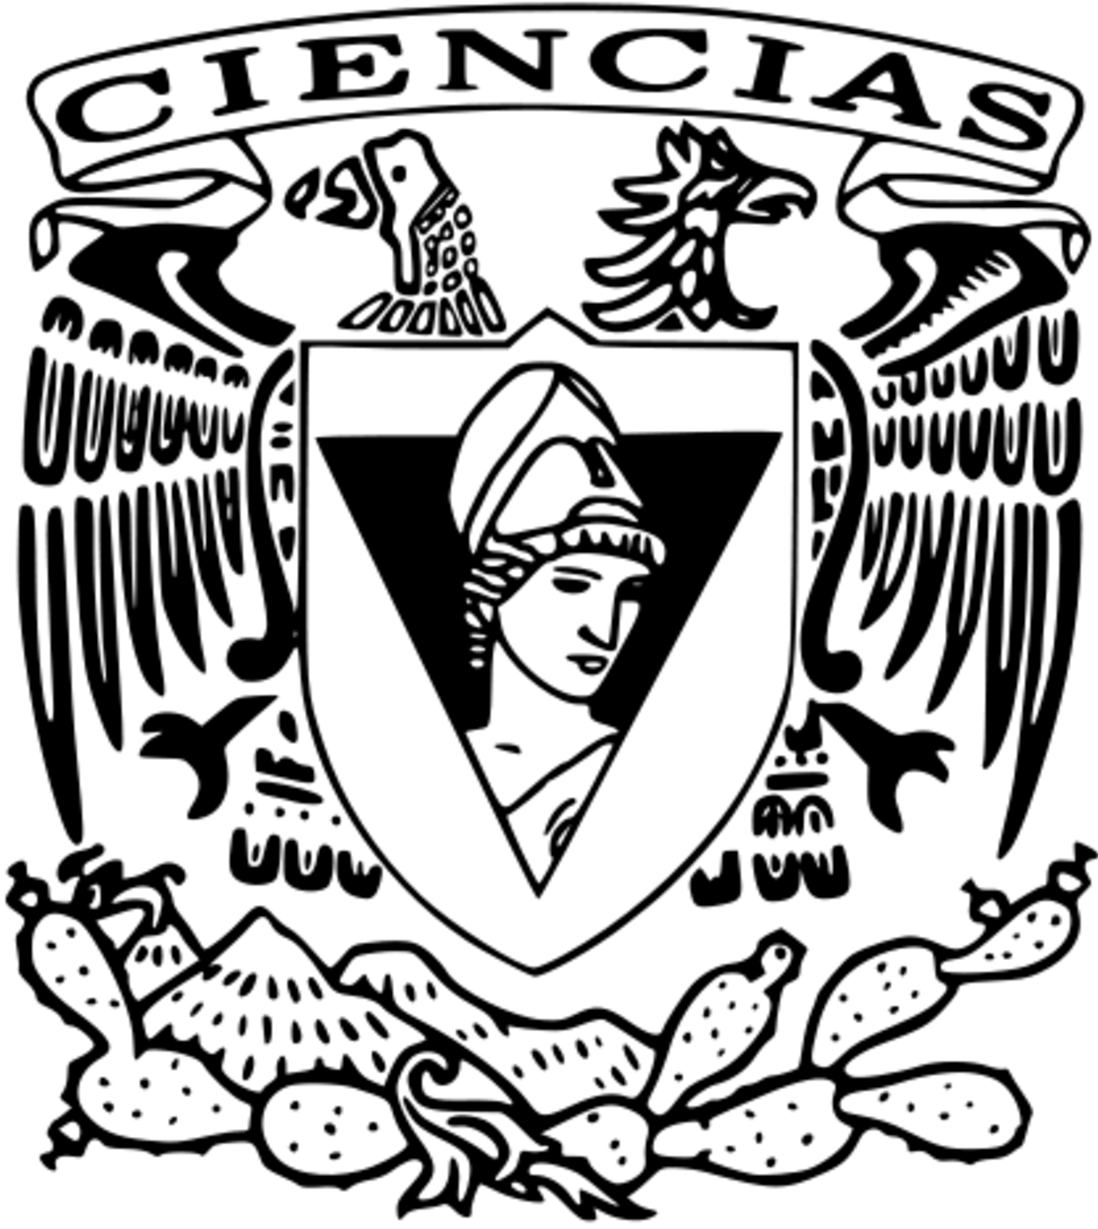
\includegraphics[height=3.4cm]{Logo_FC.png}
    	\end{center}
    \end{minipage}
\end{center}
\rule{17cm}{0.1mm}
%------ Fin de encabezado -------- %
\begin{tcolorbox}[
	title = \textcolor{black}{\textcolor{white}{Problema 1}},]
\textit{Demuestre que todo proceso estrictamente estacionario que satisface $E[X_t^2]<\infty$ para toda $t$ es tambi\'en d\'ebilmente estacionario}
\end{tcolorbox}
\begin{proof}
Para demostrar que un proceso estocástico $\{X_t\}$ estrictamente estacionario con $E[X_t^2] < \infty$ para todo $t$ es también débilmente estacionario, debemos verificar que cumple tres condiciones:

\begin{enumerate}
    \item \textbf{Segundo momento finito:}
    Por hipótesis del enunciado, $E[X_t^2] < \infty$ para todo $t \in \mathbb{Z}$.

    \item \textbf{Esperanza constante:}
    Puesto que $\{X_t\}$ es estrictamente estacionario, la función de distribución marginal $F_{X_t}(x) = P(X_t \le x)$ es idéntica para todo $t$. Por lo tanto, su esperanza matemática no depende del tiempo:
    \[
    E[X_t] = \mu \quad \forall t \in \mathbb{Z}
    \]

    \item \textbf{Autocovarianza dependiente solo del rezago $h$:}
    La distribución conjunta de cualquier par de variables $(X_t, X_{t+h})$ es invariante ante traslaciones temporales por la definición de estacionariedad estricta:
    \[
    F_{X_t, X_{t+h}}(x_1, x_2) = F_{X_{t+k}, X_{t+h+k}}(x_1, x_2) \quad \forall t, h, k \in \mathbb{Z}
    \]
    En particular, tomando el desplazamiento $k = -t$, la distribución conjunta de $(X_t, X_{t+h})$ es la misma que la de $(X_0, X_h)$. Por consiguiente:
    \[
    \gamma_X(t, t+h) = \text{Cov}(X_t, X_{t+h}) = E[X_t X_{t+h}] - E[X_t]E[X_{t+h}]
    \]
    Puesto que la distribución conjunta depende únicamente del rezago $h$:
    \[
    \gamma_X(t, t+h) = \text{Cov}(X_0, X_h) = \gamma_X(h)
    \]
\end{enumerate}

Al cumplirse las tres condiciones, se concluye que $\{X_t\}$ es un proceso **débilmente estacionario**. 
\end{proof}
\begin{tcolorbox}[
	title = \textcolor{black}{\textcolor{white}{Problema 2}},]
\textit{Sea $\{Z_t\}$ ruido blanco gaussiano $N(0,1)$ y defina 
\[
X_T = 
\begin{cases} 
Z_t& \text{si } t \text{es par} \\
\frac{Z_{t-1}^2-1}{\sqrt{2}} & \text{si } t \text{es impar}  
\end{cases}
\]}
\end{tcolorbox}
Prueba que $\{X_t\}$ es ruido blanco WN(0,1) pero que no es ruido gaussiano
\begin{proof}
Analizamos las propiedades del proceso $\{X_t\}$ definido por casos según la paridad del tiempo $t$, utilizando explícitamente las propiedades de la distribución normal y la independencia del ruido blanco gaussiano $\{Z_t\} \sim GWN(0,1)$.

\subsection*{1. Segundo momento finito ($E[X_t^2] < \infty$)}

\begin{itemize}
    \item \textbf{Si $t$ es par:} $X_t = Z_t \sim \mathcal{N}(0,1)$, por lo que:
    \[
    E[X_t^2] = E[Z_t^2] = \text{Var}(Z_t) + (E[Z_t])^2 = 1 + 0 = 1 < \infty
    \]

    \item \textbf{Si $t$ es impar:} $X_t = \frac{Z_{t-1}^2 - 1}{\sqrt{2}}$. Puesto que $Z_{t-1} \sim \mathcal{N}(0,1)$, se tiene que $E[Z_{t-1}^2] = 1$ y $E[Z_{t-1}^4] = 3$ (por la fórmula de momentos de la distribución normal centrada). Entonces:
    \[
    E[X_t^2] = E\left[\left(\frac{Z_{t-1}^2 - 1}{\sqrt{2}}\right)^2\right] = \frac{1}{2} E\left[Z_{t-1}^4 - 2Z_{t-1}^2 + 1\right] = \frac{1}{2} \left( 3 - 2(1) + 1 \right) = \frac{2}{2} = 1 < \infty
    \]
\end{itemize}
Por lo tanto, $E[X_t^2] = 1 < \infty$ para todo $t \in \mathbb{Z}$.

\subsection*{2. Esperanza matemática $E[X_t]$}

\begin{itemize}
    \item \textbf{Si $t$ es par:} 
    \[
    E[X_t] = E[Z_t] = 0
    \]

    \item \textbf{Si $t$ es impar:} 
    \[
    E[X_t] = E\left[\frac{Z_{t-1}^2 - 1}{\sqrt{2}}\right] = \frac{1}{\sqrt{2}} \left( E[Z_{t-1}^2] - 1 \right) = \frac{1}{\sqrt{2}}(1 - 1) = 0
    \]
\end{itemize}
Por ende, $E[X_t] = 0$ para todo $t \in \mathbb{Z}$ (no depende de $t$).

\subsection*{3. Función de Autocovarianza $\gamma_X(t, t+h) = E[X_t X_{t+h}]$}

\begin{itemize}
    \item \textbf{Para $h = 0$ (Varianza):}
    \[
    \gamma_X(t, t) = E[X_t^2] = 1 \quad \forall t
    \]

    \item \textbf{Para $h \neq 0$:} Analizamos los pares de subíndices según la paridad de $t$ y $t+h$:
    
    \begin{enumerate}
        \item \textbf{Ambos instantes son pares ($t$ par, $t+h$ par):}
        \[
        E[X_t X_{t+h}] = E[Z_t Z_{t+h}]
        \]
        Puesto que $h \neq 0$, $t \neq t+h$. Por ser $\{Z_t\}$ un ruido blanco gaussiano, $Z_t$ y $Z_{t+h}$ son variables aleatorias independientes, de donde $E[Z_t Z_{t+h}] = E[Z_t]E[Z_{t+h}] = 0 \cdot 0 = 0$.

        \item \textbf{Ambos instantes son impares ($t$ impar, $t+h$ impar):}
        \[
        E[X_t X_{t+h}] = E\left[\left(\frac{Z_{t-1}^2 - 1}{\sqrt{2}}\right)\left(\frac{Z_{t+h-1}^2 - 1}{\sqrt{2}}\right)\right] = \frac{1}{2} E\left[(Z_{t-1}^2 - 1)(Z_{t+h-1}^2 - 1)\right]
        \]
        Como $h \neq 0$, los instantes pasados $t-1$ y $t+h-1$ son distintos. Dado que $\{Z_t\}$ es **ruido blanco gaussiano**, $Z_{t-1}$ y $Z_{t+h-1}$ son independientes. La independencia de variables aleatorias se **preserva bajo funciones medibles**, por lo que $(Z_{t-1}^2 - 1)$ y $(Z_{t+h-1}^2 - 1)$ son también independientes. Por lo tanto:
        \[
        E[X_t X_{t+h}] = \frac{1}{2} E[Z_{t-1}^2 - 1] \cdot E[Z_{t+h-1}^2 - 1] = \frac{1}{2} (0)(0) = 0
        \]

        \item \textbf{Un instante es par y el otro es impar (sin pérdida de generalidad, $t$ par y $t+h$ impar):}
        \[
        E[X_t X_{t+h}] = E\left[Z_t \cdot \left(\frac{Z_{t+h-1}^2 - 1}{\sqrt{2}}\right)\right] = \frac{1}{\sqrt{2}} E\left[Z_t (Z_{t+h-1}^2 - 1)\right]
        \]
        \begin{itemize}
            \item Si $t \neq t+h-1$, las variables $Z_t$ y $Z_{t+h-1}$ son independientes. Por la preservación de la independencia bajo funciones medibles, $Z_t$ e $(Z_{t+h-1}^2 - 1)$ son independientes:
            \[
            E[X_t X_{t+h}] = \frac{1}{\sqrt{2}} E[Z_t] E[Z_{t+h-1}^2 - 1] = \frac{1}{\sqrt{2}} (0)(0) = 0
            \]
            \item Si $t = t+h-1$ (lo cual ocurre únicamente cuando $h = 1$), sustituimos directamente:
            \[
            E[X_t X_{t+1}] = \frac{1}{\sqrt{2}} E\left[Z_t (Z_t^2 - 1)\right] = \frac{1}{\sqrt{2}} E[Z_t^3 - Z_t] = \frac{1}{\sqrt{2}} \left( E[Z_t^3] - E[Z_t] \right)
            \]
            Dado que $Z_t \sim \mathcal{N}(0,1)$ es simétrica alrededor de cero, todos sus momentos impares son nulos, en particular $E[Z_t^3] = 0$. Por lo tanto:
            \[
            E[X_t X_{t+1}] = \frac{1}{\sqrt{2}} (0 - 0) = 0
            \]
        \end{itemize}
    \end{enumerate}
\end{itemize}

En consecuencia, la función de autocovarianza satisface:
\[
\gamma_X(h) = 
\begin{cases} 
1 & \text{si } h = 0 \\ 
0 & \text{si } h \neq 0 
\end{cases}
\]
El proceso $\{X_t\}$ es un **ruido blanco débil** $WN(0,1)$ (posee media cero, varianza constante 1 y es incorrelacionado en el tiempo), pero **NO es un Ruido Blanco Gaussiano ($GWN$)** debido a las siguientes dos razones fundamentales:
\textbf{Violación de la Distribución Gaussiana (Marginales No Gaussianas):}
    Un proceso $GWN(0,1)$ requiere obligatoriamente que $X_t \sim \mathcal{N}(0,1)$ para todo $t \in \mathbb{Z}$. Sin embargo, para cualquier instante $t$ impar:
    \[
    X_t = \frac{Z_{t-1}^2 - 1}{\sqrt{2}}
    \]
    Puesto que $Z_{t-1} \sim \mathcal{N}(0,1)$, la variable $Z_{t-1}^2$ sigue una distribución Chi-cuadrada con 1 grado de libertad ($\chi_1^2$). Por lo tanto, para $t$ impar, $X_t$ es una transformación afín de una $\chi_1^2$
\end{proof}
\begin{tcolorbox}[
	title = \textcolor{black}{\textcolor{white}{Problema 3}},]
\textit{Demuestre lo siguiente:\,\\
\begin{itemize}
    \item Encuentre la funci\'on de autocovarianza (ACV) del modelo\,\\
    \,\\
    \begin{equation*}
        X_t=Z_t+0.3Z_{t-1}-0.4Z_{t-2}\,\,\,\,\{Z_{t}\}\sim WN(0,1)
    \end{equation*}
    \item Encuentre la ACV del modelo
    \begin{equation*}
        Y_t=\bar{Z_t}-1.2\bar{Z_{t-1}}-1.6\bar{Z_{t-2}}\,\,\,\,\{\bar{Z}_{t}\}\sim WN(0,1)
    \end{equation*} 
    \item Compare ambos resultados 
\end{itemize}}
\end{tcolorbox}
\begin{proof}
Para un proceso $\text{MA}(q)$ dado por $W_t = \sum_{j=0}^{q} \theta_j \varepsilon_{t-j}$ con $\{\varepsilon_t\} \sim WN(0, \sigma^2)$ y $\theta_0 = 1$, la fórmula general de la función de autocovarianza (ACV) es:
\[
\gamma(h) = 
\begin{cases} 
\sigma^2 \displaystyle\sum_{j=0}^{q - |h|} \theta_j \theta_{j+|h|} & \text{si } |h| \le q \\ 
0 & \text{si } |h| > q 
\end{cases}
\]

\subsection*{1. ACV para el modelo $X_t = Z_t + 0.3 Z_{t-1} - 0.4 Z_{t-2}$}

Este es un proceso $\text{MA}(2)$ con $\theta_0 = 1$, $\theta_1 = 0.3$, $\theta_2 = -0.4$ y $\sigma_z^2 = 1$:

\begin{itemize}
    \item \textbf{Para $h = 0$:}
    \[
    \gamma_X(0) = 1^2 + (0.3)^2 + (-0.4)^2 = 1 + 0.09 + 0.16 = 1.25
    \]
    \item \textbf{Para $h = \pm 1$:}
    \[
    \gamma_X(\pm 1) = \theta_0 \theta_1 + \theta_1 \theta_2 = (1)(0.3) + (0.3)(-0.4) = 0.3 - 0.12 = 0.18
    \]
    \item \textbf{Para $h = \pm 2$:}
    \[
    \gamma_X(\pm 2) = \theta_0 \theta_2 = (1)(-0.4) = -0.40
    \]
    \item \textbf{Para $|h| > 2$:} $\gamma_X(h) = 0$
\end{itemize}

\subsection*{2. ACV para el modelo $Y_t = \bar{Z}_t - 1.2 \bar{Z}_{t-1} - 1.6 \bar{Z}_{t-2}$}

Este es un proceso $\text{MA}(2)$ con $\theta_0 = 1$, $\theta_1 = -1.2$, $\theta_2 = -1.6$ y $\sigma_{\bar{z}}^2 = 1$:

\begin{itemize}
    \item \textbf{Para $h = 0$:}
    \[
    \gamma_Y(0) = 1^2 + (-1.2)^2 + (-1.6)^2 = 1 + 1.44 + 2.56 = 5.00
    \]
    \item \textbf{Para $h = \pm 1$:}
    \[
    \gamma_Y(\pm 1) = (1)(-1.2) + (-1.2)(-1.6) = -1.2 + 1.92 = 0.72
    \]
    \item \textbf{Para $h = \pm 2$:}
    \[
    \gamma_Y(\pm 2) = (1)(-1.6) = -1.60
    \]
    \item \textbf{Para $|h| > 2$:} $\gamma_Y(h) = 0$
\end{itemize}

\subsection*{3. Comparación de resultados}

Si calculamos la función de autocorrelación (FAC), $\rho(h) = \frac{\gamma(h)}{\gamma(0)}$:

\begin{itemize}
    \item \textbf{Para $X_t$:} 
    \[
    \rho_X(0) = 1, \quad \rho_X(\pm 1) = \frac{0.18}{1.25} = 0.144, \quad \rho_X(\pm 2) = \frac{-0.40}{1.25} = -0.32
    \]
    \item \textbf{Para $Y_t$:} 
    \[
    \rho_Y(0) = 1, \quad \rho_Y(\pm 1) = \frac{0.72}{5.00} = 0.144, \quad \rho_Y(\pm 2) = \frac{-1.60}{5.00} = -0.32
    \]
\end{itemize}

\textbf{Conclusión:}
Aunque las funciones de autocovarianza son distintas ($\gamma_Y(h) = 4 \gamma_X(h)$ para todo $h$), la **función de autocorrelación (FAC) es idéntica** ($\rho_X(h) = \rho_Y(h)$). Esto implica que ambos modelos representan estructuras de dependencia temporal equivalentes, siendo uno el inverso no invertible del otro. 
\end{proof}
\begin{tcolorbox}[
	title = \textcolor{black}{\textcolor{white}{Problema 4}},]
\textit{Calcule la ACF y la PACF del proceso AR(2)
\begin{equation*}
    x_t=0.8\,X_{t-2}+Z_t\,\,\,\{Z_T\}\sim WN(0,\sigma^2)
\end{equation*}}
\end{tcolorbox}
\begin{proof}
\begin{enumerate}
    \item \textbf{Origen de las Ecuaciones de Yule-Walker (Ecuaciones de Recurrencia):}
    Para un proceso $\text{AR}(2)$ general $X_t = \phi_1 X_{t-1} + \phi_2 X_{t-2} + Z_t$ con $\{Z_t\} \sim WN(0,\sigma^2)$, multiplicamos la ecuación por $X_{t-k}$ (para $k \ge 0$) y tomamos esperanza matemática:
    \[
    E[X_t X_{t-k}] = \phi_1 E[X_{t-1} X_{t-k}] + \phi_2 E[X_{t-2} X_{t-k}] + E[Z_t X_{t-k}]
    \]
    Por causalidad, $Z_t$ es incorrelacionado con el pasado $X_{t-k}$ para todo $k > 0$, de donde $E[Z_t X_{t-k}] = 0$. Dividiendo toda la ecuación entre la varianza $\gamma(0)$, obtenemos las **ecuaciones de recurrencia de Yule-Walker** para la autocorrelación $\rho(k) = \frac{\gamma(k)}{\gamma(0)}$:
    \[
    \rho(k) = \phi_1 \rho(k-1) + \phi_2 \rho(k-2), \quad \text{para } k \ge 1
    \]
    Para nuestro proceso específico $X_t = 0.8 X_{t-2} + Z_t$, identificamos los parámetros:
    \[
    \phi_1 = 0, \quad \phi_2 = 0.8
    \]
    Por lo tanto, la ecuación de recurrencia simplificada es:
    \[
    \rho(k) = 0.8 \, \rho(k-2), \quad \text{para } k \ge 1
    \]

    \item \textbf{Cálculo de la Función de Autocorrelación (ACF):}
    Sabiendo que por definición $\rho(0) = 1$, aplicamos la condición inicial para $k = 1$:
    \[
    \rho(1) = 0.8 \, \rho(1 - 2) = 0.8 \, \rho(-1)
    \]
    Dado que la ACF es simétrica ($\rho(-1) = \rho(1)$), se tiene que $\rho(1) = 0.8 \, \rho(1) \implies \rho(1)(1 - 0.8) = 0 \implies \rho(1) = 0$.

    A partir de las condiciones iniciales $\rho(0) = 1$ y $\rho(1) = 0$, resolvemos la recurrencia para paridad de $k$:
    \begin{itemize}
        \item \textbf{Para rezagos pares ($k = 2m$):}
        \[
        \rho(2) = 0.8 \, \rho(0) = 0.8, \quad \rho(4) = 0.8 \, \rho(2) = (0.8)^2, \quad \dots \quad \rho(2m) = (0.8)^m
        \]
        \item \textbf{Para rezagos impares ($k = 2m + 1$):}
        \[
        \rho(3) = 0.8 \, \rho(1) = 0, \quad \dots \quad \rho(2m+1) = 0
        \]
    \end{itemize}
    En resumen, la función de autocorrelación $\rho(k)$ es:
    \[
    \rho(k) = 
    \begin{cases} 
    (0.8)^{k/2} & \text{si } k \text{ es par} \\ 
    0 & \text{si } k \text{ es impar} 
    \end{cases}
    \]

    \item \textbf{Cálculo de la Función de Autocorrelación Parcial (PACF):}
    La autocorrelación parcial $\phi_{kk}$ mide la correlación entre $X_t$ y $X_{t-k}$ tras eliminar el efecto de las variables intermedias. Por ser un proceso puramente autorregresivo de orden $p = 2$ ($\text{AR}(2)$):
    \begin{itemize}
        \item \textbf{Para $k = 1$:} $\phi_{11} = \rho(1) = 0$.
        \item \textbf{Para $k = 2$:} $\phi_{22} = \phi_2 = 0.8$.
        \item \textbf{Para $k \ge 3$:} La PACF de un proceso $\text{AR}(p)$ se corta exactamente después del rezago $p$, por lo que $\phi_{kk} = 0$ para todo $k \ge 3$.
    \end{itemize}
    En resumen, la función de autocorrelación parcial $\phi_{kk}$ es:
    \[
    \phi_{kk} = 
    \begin{cases} 
    0 & \text{si } k = 1 \\ 
    0.8 & \text{si } k = 2 \\ 
    0 & \text{si } k \ge 3 
    \end{cases}
    \]
\end{enumerate}
\end{proof}
\begin{tcolorbox}[
	title = \textcolor{black}{\textcolor{white}{Problema 5}},]
\textit{Determine cu\'ales de los siguientes pocesos ARMA (p,q) son causales y cu\'ales son invertibles en cada caso $\{Z_t\}\sim WN(0,1)$
\begin{itemize}
    \item $X_t+0.2X_{t-1}-0.48X_{t-2}=Z_t$
    \item $X_t+1.9X_{t-1}+0.88X_{t-2}=Z_t+0.2Z_{t-1}+0.7Z_{t-2}$
    \item $X_t+0.6X_{t-1}=Z_t+1.2Z_{t-1}$
    \item $X_t+1.8X_{t-1}+0.81X_{t-2}=Z_t$
    \item $X_t+1.6X_{t-1}=Z_t-0.4Z_t+0.04Z_{t-2}$
    \item $X_{t}=0.80X_{t-1}-0.15X_{t-2}+Z_t-0.30Z_{t-1}$
    \item $X_t=X_{t-1}-0.50X_{t-2}+Z_t-Z_{t-1}$
\end{itemize}}
\end{tcolorbox}
\begin{proof}
Para determinar si un proceso $\text{ARMA}(p,q)$ definido por $\phi(B)X_t = \theta(B)Z_t$ es \textbf{causal} e \textbf{invertible}, analizamos las raíces de los polinomios autorregresivo $\phi(z) = 0$ y de medias móviles $\theta(z) = 0$:

\begin{itemize}
    \item \textbf{Causalidad:} Todas las raíces de $\phi(z) = 0$ deben estar **estrictamente fuera** del disco unidad ($|z| > 1$).
    \item \textbf{Invertibilidad:} Todas las raíces de $\theta(z) = 0$ deben estar **estrictamente fuera** del disco unidad ($|z| > 1$).
\end{itemize}

Para polinomios de segundo grado $1 + a_1 z + a_2 z^2 = 0$, la condición equivalente a que sus raíces estén fuera del disco unidad es cumplir las tres condiciones del triángulo de estabilidad:
\[
1) \quad |a_2| < 1, \qquad 2) \quad a_2 + a_1 > -1, \qquad 3) \quad a_2 - a_1 > -1
\]

A continuación se analiza cada inciso:

\begin{enumerate}
    \item $X_t + 0.2 X_{t-1} - 0.48 X_{t-2} = Z_t$
    \begin{itemize}
        \item \textbf{Causalidad:} $\phi(z) = 1 + 0.2z - 0.48z^2 = 0$. Resolviendo:
        \[
        z = \frac{-0.2 \pm \sqrt{0.04 - 4(-0.48)(1)}}{-0.96} = \frac{-0.2 \pm 1.4}{-0.96} \implies z_1 = -1.25, \quad z_2 = \frac{5}{3} \approx 1.67
        \]
        Como $|z_1| = 1.25 > 1$ y $|z_2| \approx 1.67 > 1$, el proceso es \textbf{causal}.
        \item \textbf{Invertibilidad:} $\theta(z) = 1$, no tiene raíces finitas. Es \textbf{invertible}.
    \end{itemize}

    \item $X_t + 1.9 X_{t-1} + 0.88 X_{t-2} = Z_t + 0.2 Z_{t-1} + 0.7 Z_{t-2}$
    \begin{itemize}
        \item \textbf{Causalidad:} $\phi(z) = 1 + 1.9z + 0.88z^2 = 0$.
        Verificamos las condiciones de estabilidad: $a_2 = 0.88 < 1$, $0.88 + 1.9 = 2.78 > -1$, y $0.88 - 1.9 = -1.02 \ngtr -1$. Como la tercera condición no se cumple, al menos una raíz tiene $|z| \le 1$. No es \textbf{causal}.
        \item \textbf{Invertibilidad:} $\theta(z) = 1 + 0.2z + 0.7z^2 = 0$.
        Verificamos: $a_2 = 0.7 < 1$, $0.7 + 0.2 = 0.9 > -1$, $0.7 - 0.2 = 0.5 > -1$. Se cumplen las tres condiciones. Es \textbf{invertible}.
    \end{itemize}

    \item $X_t + 0.6 X_{t-1} = Z_t + 1.2 Z_{t-1}$
    \begin{itemize}
        \item \textbf{Causalidad:} $\phi(z) = 1 + 0.6z = 0 \implies z = -1 / 0.6 = -5/3 \approx -1.67$.
        Como $|z| \approx 1.67 > 1$, es \textbf{causal}.
        \item \textbf{Invertibilidad:} $\theta(z) = 1 + 1.2z = 0 \implies z = -1 / 1.2 = -5/6 \approx -0.83$.
        Como $|z| \approx 0.83 \le 1$, no es \textbf{invertible}.
    \end{itemize}

    \item $X_t + 1.8 X_{t-1} + 0.81 X_{t-2} = Z_t$
    \begin{itemize}
        \item \textbf{Causalidad:} $\phi(z) = 1 + 1.8z + 0.81z^2 = (1 + 0.9z)^2 = 0 \implies z = -10/9 \approx -1.11$.
        Como $|z| \approx 1.11 > 1$, es \textbf{causal}.
        \item \textbf{Invertibilidad:} $\theta(z) = 1$, no tiene raíces finitas. Es \textbf{invertible}.
    \end{itemize}

    \item $X_t + 1.6 X_{t-1} = Z_t - 0.4 Z_{t-1} + 0.04 Z_{t-2}$
    \begin{itemize}
        \item \textbf{Causalidad:} $\phi(z) = 1 + 1.6z = 0 \implies z = -1 / 1.6 = -0.625$.
        Como $|z| = 0.625 \le 1$, no es \textbf{causal}.
        \item \textbf{Invertibilidad:} $\theta(z) = 1 - 0.4z + 0.04z^2 = (1 - 0.2z)^2 = 0 \implies z = 1 / 0.2 = 5$.
        Como $|z| = 5 > 1$, es \textbf{invertible}.
    \end{itemize}

    \item $X_t - 0.80 X_{t-1} + 0.15 X_{t-2} = Z_t - 0.30 Z_{t-1}$
    \begin{itemize}
        \item \textbf{Causalidad:} $\phi(z) = 1 - 0.80z + 0.15z^2 = (1 - 0.5z)(1 - 0.3z) = 0 \implies z_1 = 2, z_2 = 10/3 \approx 3.33$.
        Como $|z_1| > 1$ y $|z_2| > 1$, es \textbf{causal}.
        \item \textbf{Invertibilidad:} $\theta(z) = 1 - 0.30z = 0 \implies z = 10/3 \approx 3.33$.
        Sin embargo, observamos que existe cancelación de factores comunes entre $\phi(z)$ y $\theta(z)$ en $(1 - 0.3z)$. Simplificando el modelo queda $X_t - 0.5 X_{t-1} = Z_t$, el cual sigue siendo \textbf{causal} y es trivialmente \textbf{invertible}.
    \end{itemize}

    \item $X_t - X_{t-1} + 0.50 X_{t-2} = Z_t - Z_{t-1}$
    \begin{itemize}
        \item \textbf{Causalidad:} $\phi(z) = 1 - z + 0.50z^2 = 0$.
        Verificamos estabilidad: $a_2 = 0.5 < 1$, $0.5 - 1 = -0.5 > -1$, $0.5 - (-1) = 1.5 > -1$. Las raíces complejas conjugadas son $z = 1 \pm i$, con módulo $|z| = \sqrt{1^2 + 1^2} = \sqrt{2} \approx 1.414 > 1$. Es \textbf{causal}.
        \item \textbf{Invertibilidad:} $\theta(z) = 1 - z = 0 \implies z = 1$.
        Puesto que la raíz está exactamente sobre el círculo unitario ($|z| = 1$), el proceso no es \textbf{invertible}.
    \end{itemize}
\end{enumerate}
\end{proof}
\begin{tcolorbox}[
	title = \textcolor{black}{\textcolor{white}{Problema 6}},]
\textit{Demuestre que un proceso AR(1) dado por $X_t=\theta X_{t-1}+Z_{t}$ es estacionario de segundo orden si $|\theta|<1$}
\end{tcolorbox}
\begin{proof}
    Es claro que al iterar $k$ veces obtenemos que $X_t=\phi^kX_{t-k}+\sum_{j=0}^{k-1}\phi^jZ_{t-j}$, como $|\phi|<1$ y $E(X^2_{t})<\infty$ entonces el termino $\phi^kY_{t-k}\to 0$ en media cuadratica, por tanto podemos suponer que
    \begin{equation*}
        Y_t=\sum_{j=0}^\infty \phi^jZ_{t-j}
    \end{equation*}\,\\
    \begin{enumerate}
        \item Consideramos el proceso $\text{AR}(1)$ dado por $X_t = \theta X_{t-1} + Z_t$ para $t \ge 1$, donde $\{Z_t\} \sim WN(0, \sigma_z^2)$ y $|\theta| < 1$. 

Asumiendo que el estado inicial $X_0$ satisface que su segundo momento es finito, es decir, $E[X_0^2] = C_0 < \infty$, demostraremos por **inducción matemática** que $E[X_t^2] < \infty$ para todo $t \ge 1$.

\subsection*{Paso Inductivo: Acotamiento de Segundos Momentos}

\begin{enumerate}
    \item \textbf{Base de la inducción ($t = 0$):}
    Por hipótesis, $E[X_0^2] = C_0 < \infty$.

    \item \textbf{Hipótesis inductiva:}
    Supongamos que para un instante $t - 1 \ge 0$ se cumple que $E[X_{t-1}^2] < \infty$.

    \item \textbf{Paso de inducción ($t$):}
    Elevando al cuadrado la ecuación del proceso $X_t = \theta X_{t-1} + Z_t$:
    \[
    X_t^2 = (\theta X_{t-1} + Z_t)^2 = \theta^2 X_{t-1}^2 + 2\theta X_{t-1}Z_t + Z_t^2
    \]
    Aplicando esperanza matemática en ambos lados:
    \[
    E[X_t^2] = \theta^2 E[X_{t-1}^2] + 2\theta E[X_{t-1} Z_t] + E[Z_t^2]
    \]
    Puesto que $Z_t$ es un ruido blanco no correlacionado con el pasado $X_{t-1}$, tenemos que $E[X_{t-1} Z_t] = E[X_{t-1}] E[Z_t] = 0$. Además, $E[Z_t^2] = \sigma_z^2 < \infty$. Por lo tanto:
    \[
    E[X_t^2] = \theta^2 E[X_{t-1}^2] + \sigma_z^2
    \]
    Por la hipótesis inductiva, $E[X_{t-1}^2] < \infty$. Como $\theta^2 < 1$ y $\sigma_z^2 < \infty$, la suma de estos dos términos finitos da como resultado un valor finito:
    \[
    E[X_t^2] < \infty
    \]
\end{enumerate}

Por el principio de inducción matemática, $E[X_t^2] < \infty$ para todo $t \ge 0$.
        \item Para calcular la esperanza de $Y_t$ primero veamos que como $E(|Z_{t-j}|)\leq E(Z_{t-j})^2=\sigma^2$, tenemos que:\,\\
        \begin{equation*}
            E\left(\sum_{j=0}^n |\theta|^j|Z_{t-j}|\right)=\sum_{i=0}^n |\theta|^jE(|Z_{t-j}|)\leq \sum_{j=0}^n |\theta|^j
        \end{equation*}
        Por tanto como $|\theta|<1$ la serie derecha converge es decir:\,\\
        \begin{equation*}
            E\left(\sum_{j=0}^\infty|\theta|^j|Z_{t-j}|\right)<\infty
        \end{equation*}
        Ahora como claramente:\,\\
        \begin{equation*}
            \left|\sum_{j=0}^n \theta^jZ_{t-j}\right|\leq \sum_{j=0}^n |\theta|^j|Z_{t-j}|\leq \sum_{j=0}^\infty|\theta|^j|Z_{t-j}|=Y
        \end{equation*}\,\\
        Como ya demostramos que $E(y)< \infty$ por convergencia dominada tenemos que:\,\\
        \begin{equation*}
            E(Y_t)=E\left(\lim_{n\to\infty}\sum_{i=1}^n \theta^jZ_{t-j}\right)=\lim_{n\to \infty}\sum_{j=0}^\infty |\theta|^jE(Z_{t-j})=0
        \end{equation*}, por tanto la esperanza no depende de $t$
        \item En este paso voy a suponer que la puedo meter y sacar el l\'imite de la covarianza libremente, lo cual es cierto, se puede mostrar de nuevo usando convergencia dominada acotando por un producto de cauchy pero, esta engorroso de escribir, tomamos $h>0$:\,\\
        \begin{equation*}
            \gamma(h)=cov\left(\sum_{j=0}^\infty\theta^jZ_{t+h-j},\sum_{k=0}^\infty\theta^jZ_{t-k}\right)=\sum_{j=0}^\infty\sum_{k=0}^{\infty}\theta^j\theta^kcov(Z_{t+h-j}Z_{t-k})
        \end{equation*}\,\\
        de nuevo $cov(Z_{t+h-j},Z_{t-k})\neq 0$ si y solo si $t+h-j=t-k\implies k=h+j$, por tanto reescribimos:\,\\
        \begin{equation*}
            \gamma(h)=\sum_{j=0}^{\infty} \theta^j\theta^{j+h}\sigma^2=\frac{\sigma^2 \theta^h}{1-\theta^2}
        \end{equation*}\,\\
        De nuevo extendemos para $h<0\implies -h>0$ $\gamma(-h)=\gamma(h)$ por tanto en general:\,\\
        \begin{equation*}
            \gamma(h)=\frac{\sigma^2\theta^{|h|}}{1-\theta^2}
        \end{equation*}
    \end{enumerate}
\end{proof}
\begin{tcolorbox}[
	title = \textcolor{black}{\textcolor{white}{Problema 7}},]
\textit{Suponga que $X_t$ es un proceso lineal, es decir:\,\\
\begin{equation*}
    X_t=\sum_{j=-\infty}^\infty \phi_jZ_{t-j}\,\,\,\,\{Z_T\}\sim WN(0,1)\,\,\,\,\sum_{j=-\infty}^{\infty}\,|\phi_j|<\infty
\end{equation*}
Demuestre:\,\\
\begin{equation*}
    \sum_{h=-\infty}^{\infty}\,\,\,|\gamma(h)|<\infty
\end{equation*}}
\end{tcolorbox}
\begin{proof}
    Sabemos que $\gamma(h)=\sigma^2_{\omega}\sum_{j=-\infty}^\infty\,\phi_{j+h}\phi_{j}$, veamos que como $\gamma(-h)=\gamma(h)\implies |\gamma(-h)|=|\gamma(h)|$:\,\\
    \begin{equation*}
        \sum_{h=-\infty}^\infty |\gamma(h)|=\sum_{h=-\infty}^{\infty}|\gamma(-h)|=\sum_{h=-\infty}^{\infty}\sigma^2\left|\sum_{j=-\infty}^\infty \phi_{j}\phi_{j-h}\right|\leq \sum_{h=-\infty}^{\infty}\sigma^2 \sum_{j=-\infty}^\infty |\phi_{j}||\phi_{j-h}|=\sigma^2\left(\sum_{j=-\infty}^\infty\,|\phi_j|\right)\left(\sum_{j=-\infty}^\infty\,|\phi_j|\right)
    \end{equation*}\,\\
    \,\\
    Como $\displaystyle\sum_{j=-\infty}^\infty |\phi_j|\leq \infty$ es absulatamente convergente el producto de Cauchy  $\left(\displaystyle\sum_{j=-\infty}^\infty\,|\phi_j|\right)\left(\displaystyle\sum_{j=-\infty}^\infty\,|\phi_j|\right)\leq \infty$\,\\
    \,\\
    Por tanto $\displaystyle \sum_{j=-\infty}^{\infty}\,|\gamma(h)|\leq \infty$
\end{proof}

\begin{tcolorbox}[
	title = \textcolor{black}{\textcolor{white}{Problema 8}},]
\textit{Suponga que $X_t=\mu+Z_t+\theta Z_{t-1}$ donde $Z_t\sim WN(0,\sigma_z^2)$
\begin{itemize}
    \item Demuestre que $E(X_t)=\mu$ para toda $t$
    \item Demuestre que la funci\'on de autocovarianza de $X_t$ est\'a dada por:\,\\
    \begin{equation*}
        \gamma_{X}(0)=\sigma_{z}^2(1+\theta^2)\,\,\,\gamma_{X}(\pm 1)=\sigma_{z}^2\theta
    \end{equation*}
\end{itemize}}
\end{tcolorbox}
\begin{proof}

\subsection*{1. Esperanza matemática $E(X_t) = \mu$}

Dado el modelo $X_t = \mu + Z_t + \theta Z_{t-1}$, aplicamos el operador esperanza:
\[
E(X_t) = E(\mu + Z_t + \theta Z_{t-1}) = E(\mu) + E(Z_t) + \theta E(Z_{t-1})
\]

Como $Z_t \sim WN(0, \sigma_z^2)$, se tiene que $E(Z_t) = E(Z_{t-1}) = 0$. Por lo tanto:
\[
E(X_t) = \mu + 0 + \theta(0) = \mu \quad \forall t
\]

\subsection*{2. Autocovarianza mediante la fórmula de $\text{MA}(q)$}

El proceso $X_t - \mu = Z_t + \theta Z_{t-1}$ corresponde a un $\text{MA}(1)$ con coeficientes $\theta_0 = 1$ y $\theta_1 = \theta$.

La fórmula general para la autocovarianza de un proceso $\text{MA}(q)$ a un rezago $h$ es:
\[
\gamma_X(h) = 
\begin{cases} 
\sigma_z^2 \displaystyle\sum_{j=0}^{q - |h|} \theta_j \theta_{j+|h|} & \text{si } |h| \le q \\ 
0 & \text{si } |h| > q 
\end{cases}
\]

Aplicando la fórmula para $q = 1$:

\begin{itemize}
    \item \textbf{Para $h = 0$:}
    \[
    \gamma_X(0) = \sigma_z^2 \sum_{j=0}^{1} \theta_j^2 = \sigma_z^2 (\theta_0^2 + \theta_1^2) = \sigma_z^2(1 + \theta^2)
    \]

    \item \textbf{Para $h = \pm 1$:}
    Por simetría, $\gamma_X(1) = \gamma_X(-1)$:
    \[
    \gamma_X(\pm 1) = \sigma_z^2 \sum_{j=0}^{0} \theta_j \theta_{j+1} = \sigma_z^2 (\theta_0 \theta_1) = \sigma_z^2 \theta
    \]
\end{itemize}

Por lo tanto:
\[
\gamma_X(0) = \sigma_z^2(1 + \theta^2) \quad \text{y} \quad \gamma_X(\pm 1) = \sigma_z^2 \theta 
\]
\end{proof}

\begin{tcolorbox}[
	title = \textcolor{black}{\textcolor{white}{Problema 9}},]
\textit{Para un proceso $\{Z_t\}\sim WN(0,1)$ con $t\in \Z$ considere la serie:\,\\
\begin{equation*}
    X_t=Z_{t}Z_{t-1}
\end{equation*}
Determine la media y la funci\'on de autocovarianza de $X_t$, e indique si el proceso es estacionario de segundo orden}
\end{tcolorbox}
\begin{proof}
Para determinar si el proceso $X_t = Z_t Z_{t-1}$ es estacionario de segundo orden (o débilmente estacionario), calculamos su media, varianza y función de autocovarianza. 

Dado que $\{Z_t\} \sim WN(0, 1)$, se cumple que $E(Z_t) = 0$, $E(Z_t^2) = 1$ para todo $t$, y $E(Z_t Z_s) = 0$ cuando $t \neq s$.

\begin{enumerate}
    \item \textbf{Esperanza matemática $E(X_t)$:}
    Puesto que $Z_t$ y $Z_{t-1}$ corresponden a instantes de tiempo distintos dentro de un ruido blanco, son variables incorrelacionadas:
    \[
    E(X_t) = E(Z_t Z_{t-1}) = E(Z_t) E(Z_{t-1}) = 0 \cdot 0 = 0 \quad \forall t
    \]
    La media es constante e igual a cero.

    \item \textbf{Función de Autocovarianza $\gamma_X(h)$:}
    Calculamos $\gamma_X(h) = \text{Cov}(X_t, X_{t+h}) = E(X_t X_{t+h}) - E(X_t)E(X_{t+h}) = E(X_t X_{t+h})$ para los distintos rezagos $h \ge 0$:

    \begin{itemize}
        \item \textbf{Para $h = 0$ (Varianza):}
        \[
        \gamma_X(0) = E(X_t^2) = E(Z_t^2 Z_{t-1}^2) = E(Z_t^2) E(Z_{t-1}^2) = 1 \cdot 1 = 1 < \infty
        \]

        \item \textbf{Para $h = 1$:}
        \[
        \gamma_X(1) = E(X_t X_{t+1}) = E(Z_t Z_{t-1} \cdot Z_{t+1} Z_t) = E(Z_{t+1} Z_t^2 Z_{t-1})
        \]
        Puesto que $Z_{t+1}$ es incorrelacionado con $Z_t^2 Z_{t-1}$ pues al ser ruido blanco gaussiano la estacionariedad debil implica la fuerte (independencia y misma distribucion):
        \[
        \gamma_X(1) = E(Z_{t+1}) E(Z_t^2 Z_{t-1}) = 0 \cdot E(Z_t^2 Z_{t-1}) = 0
        \]

        \item \textbf{Para $h \ge 2$:}
        En el producto $X_t X_{t+h} = Z_t Z_{t-1} Z_{t+h} Z_{t+h-1}$, el término con el índice de tiempo más reciente $Z_{t+h}$ no comparte subíndice con ningún otro factor. Por incorrelación:
        \[
        \gamma_X(h) = E(Z_{t+h}) E(Z_{t+h-1} Z_t Z_{t-1}) = 0 \cdot E(Z_{t+h-1} Z_t Z_{t-1}) = 0
        \]
    \end{itemize}

    Por simetría, $\gamma_X(h) = \gamma_X(-h)$. Así, la función de autocovarianza es:
    \[
    \gamma_X(h) = 
    \begin{cases} 
    1 & \text{si } h = 0 \\ 
    0 & \text{si } h \neq 0 
    \end{cases}
    \]

    \item \textbf{Estacionariedad de segundo orden:}
    \begin{itemize}
        \item El segundo momento es finito: $E(X_t^2) = 1 < \infty$ para todo $t$.
        \item La media es constante: $E(X_t) = 0$ para todo $t$.
        \item La autocovarianza $\gamma_X(h)$ solo depende del rezago $h$ y no del tiempo $t$.
    \end{itemize}

    Por lo tanto, el proceso $X_t$ **sí es estacionario de segundo orden** (de hecho, su función de autocovarianza es idéntica a la de un ruido blanco $WN(0,1)$).
\end{enumerate}
\end{proof}
\begin{tcolorbox}[
	title = \textcolor{black}{\textcolor{white}{Problema 10}},]
\textit{Para un proceso:\,\\
\begin{equation*}
    X_t=Z_{t-1}+2Z_{t}+Z_{t+1}
\end{equation*}
Donde los $Z_t$ son independientes con media cero y varianza $\sigma_x^2$, determine las funcines de autocovarianza y autocorrelaci\'on y gracique la ACF como funci\'on de h}
\end{tcolorbox}
\begin{proof}

\subsection*{1. Reescritura del modelo como un proceso $\text{MA}(q)$}

Reordenando los términos en orden cronológico, la serie $X_t$ se expresa como:
\[
X_t = Z_{t+1} + 2 Z_t + Z_{t-1}
\]

Si definimos el desfase de tiempo sustituyendo el índice por $t' = t + 1$, observamos que $X_t$ es una suma finita de variables independientes desplazadas en el tiempo, lo que equivale a un proceso de Medias Móviles de orden $q = 2$ (ó visto a través de $3$ términos consecutivos).

Definiendo la representación estándar $X_t = \sum_{j=0}^{2} \theta_j \varepsilon_{t+1-j}$ con los coeficientes:
\[
\theta_0 = 1, \quad \theta_1 = 2, \quad \theta_2 = 1, \quad \text{y} \quad \text{Var}(Z_t) = \sigma_z^2
\]

La fórmula general de autocovarianza para una combinación lineal de este tipo con rezago $h$ es:
\[
\gamma_X(h) = 
\begin{cases} 
\sigma_z^2 \displaystyle\sum_{j=0}^{q - |h|} \theta_j \theta_{j+|h|} & \text{si } |h| \le q \\ 
0 & \text{si } |h| > q 
\end{cases}
\]

\subsection*{2. Cálculo de la Función de Autocovarianza (ACV) y Autocorrelación (ACF)}

Aplicando la fórmula para $q = 2$:

\begin{itemize}
    \item \textbf{Para $h = 0$ (Varianza):}
    \[
    \gamma_X(0) = \sigma_z^2 (\theta_0^2 + \theta_1^2 + \theta_2^2) = \sigma_z^2 (1^2 + 2^2 + 1^2) = 6 \sigma_z^2
    \]

    \item \textbf{Para $h = \pm 1$:}
    \[
    \gamma_X(\pm 1) = \sigma_z^2 (\theta_0 \theta_1 + \theta_1 \theta_2) = \sigma_z^2 (1 \cdot 2 + 2 \cdot 1) = 4 \sigma_z^2
    \]

    \item \textbf{Para $h = \pm 2$:}
    \[
    \gamma_X(\pm 2) = \sigma_z^2 (\theta_0 \theta_2) = \sigma_z^2 (1 \cdot 1) = \sigma_z^2
    \]

    \item \textbf{Para $|h| \ge 3$:}
    \[
    \gamma_X(h) = 0
    \]
\end{itemize}

Dividiendo entre $\gamma_X(0) = 6 \sigma_z^2$, la función de autocorrelación $\rho_X(h) = \frac{\gamma_X(h)}{\gamma_X(0)}$ resulta:
\[
\rho_X(h) = 
\begin{cases} 
1 & \text{si } h = 0 \\
\frac{4}{6} = \frac{2}{3} & \text{si } h = \pm 1 \\
\frac{1}{6} & \text{si } h = \pm 2 \\
0 & \text{si } |h| \ge 3
\end{cases}
\]

\subsection*{3. Argumentación sobre el uso de la propiedad de Ruido Blanco}

El hecho de que $\{Z_t\}$ sea un **ruido blanco** es precisamente lo que permite aplicar la fórmula del proceso $\text{MA}$:

1. **Incorrelación de $Z_t$:** Como $\text{Cov}(Z_t, Z_s) = 0$ para $t \neq s$, al calcular $\text{Cov}(X_t, X_{t+h})$ todos los productos cruzados $E[Z_t Z_s]$ se anulan, sobreviviendo únicamente los términos donde los índices coinciden.
2. **Homocedasticidad:** Dado que $E[Z_t^2] = \sigma_z^2$ para todo $t$, la varianza de $X_t$ y sus autocovarianzas son constantes e independientes del tiempo $t$.
3. **Estacionariedad de $X_t$:** Al ser $\{Z_t\}$ ruido blanco, $X_t$ resulta ser un proceso débilmente estacionario con media $E[X_t] = 0$ y una ACF que se corta después del rezago $h = 2$. 

\end{proof}
\begin{tcolorbox}[
	title = \textcolor{black}{\textcolor{white}{Problema 11}},]
\textit{Considere el modelo:\,\\
\begin{equation*}
    X_t=\beta_1+\beta_2t+Z_t
\end{equation*}
donde $\beta_1$ y $\beta_2$ son constantes y $Z_t\sim WN(0,1)$}
\begin{itemize}
    \item Determine si $X_t$ es estacionario
    \item Demuestre que el proceso $Y_t=X_t-X_{t-1}$
    \item Demuestre que el proceso $Y_t=X_t-X_{t-1}$ es estacionario
    \item Demuestre que el promedio m\'ovil cumple que:\,\\
    \begin{equation*}
        E(v_t)=E\left(\frac{1}{2q+1}\sum_{j=-q}^q x_{t-j}\right)=\beta_1+\beta_2l
    \end{equation*}
    \item Resuma en palabras las implicaciones de los incisos anteriores, considerando la forma del modelo inicial 
\end{itemize}
\end{tcolorbox}
\begin{proof}
    \begin{itemize}
        \item Claramente $X_t$ no es estacionario pues $E(x_t)=E(\beta_1+\beta_2t+Z_t)=\beta_1+\beta_2t+E(Z_t)=\beta_1+\beta_2t$ la cual claraamente depende de $t$
        \item Notemos que $X_{t}-X_{t-1}=\beta_1+\beta_2(t)+Z_{t}-\beta_1-(t-1)\beta_2+Z_{t-1}=\beta_2+Z_{t}+Z_{t-1}$ claramente $var(Y_t)=var(Z_{t})+var(z_{t-1})+cov(z_{t},z_{t-1})=1+1$, por tanto el segundo momento es finito,
        luego $E(Y_t)=\beta_2+E(Z_t)+E(Z_{t-1})=\beta_2$ por tanto la esperanza no depende de $t$, ahora $T_t$ es AM(2) por tanto su ACV sigue la formula del problema 13, la cual claramente solo depende de $h$, es decir $Y_t$ es estacionario de segundo orden
        \item Veamos que:\,\\
        \begin{align*}
            E(v_l)&=E\left(\frac{1}{2q+1}\sum_{j=-q}^q \beta_1+\beta_2(l-j)+Z_{l-j}\right)\,\\
            \,\\&=\frac{1}{2q+1}+\sum_{j=-q}^q \beta_1+\beta_2(l-j)+E(Z_t)=\frac{1}{2q+1}((2q+1)\beta_1+\beta_2\sum_{j=-q}^{q}(l-q))=\beta_1+\beta_2l
        \end{align*}
        \item Sea $ X_t=\beta_1+\beta_2t+Z_t$ con $\{Z_t\}\sim WN(0,1)$ entonces $X_t$ no es estacionario, entonces $X_{t}-X_{t-1}$ es AM(2), por tanto es estacionario, y sea $v_l$ el promedio de medias moviles entonces $E(v_l)=\beta_1+\beta_2l$
    \end{itemize}
\end{proof}


\begin{tcolorbox}[
	title = \textcolor{black}{\textcolor{white}{Problema 13}},]
\textit{Demostrar que la ACV de un proceso MA(q) es dada por
\[
\gamma(k) = 
\begin{cases} 
\sigma^2\sum_{j=0}^{q-|k|}\theta_j\theta_{j+|k|}& \text{si } |k|\leq q \\
0 & \text{si } |k|>q 
\end{cases}
\]
donde $\theta_0:=1$ y $\theta_j:=0$ cuando $j>q$}
\end{tcolorbox}
\begin{proof}
    Por definici\'on:\,\\
    \begin{equation*}
        \gamma(k)=cov(x_{k+h},x_h)=cov\left(\mu+\sum_{i=0}^q\theta_i\epsilon_{k+h-i},\mu+\sum_{j=0}^q\theta_j\epsilon_{h-j}\right)
    \end{equation*}
    Con $\{\epsilon\}\sim WM(0,1)$, usando las propiedades de la covarianza:\,\\
    \begin{equation*}
        \gamma(k)=\sum_{i=0}^q\sum_{j=0}^q\theta_i\theta_j\,cov(\epsilon_{k+h-i},\epsilon_{h-j})
    \end{equation*}
    Aplicando la propiedad del ruido blanco:\,\\
    \begin{equation*}
        cov(\epsilon_i,\epsilon_j)= 
    \begin{cases} 
        0& \text{si } i\neq j\\
        \sigma^2 & \text{si } i 
    \end{cases}
    \end{equation*}
    Tenemos que $cov(\epsilon_{k+h-i},\epsilon_{k-j})\neq 0$ si y solo si $k+h-i=h-j\implies k+j=i$, temos que $0\leq i\leq q$, suponemos $k\geq 0$ es claro que si $k>q$ entonces $i\geq k$ lo cual es imposible, por tanto si $|k|>q$ entonces
    $cov(\epsilon_{k+h-i},\epsilon_{k-j})=0$ para todo $i,j\in \{1,2,\cdots,q\}$, ahora si $k\leq q$, podemos reescribir:\,\\
    \begin{equation*}
        \gamma(k)=\sum_{j=0}^q\theta_{j}\theta_{j+k}cov(\epsilon_{h-j},\epsilon_{h-j})=\sigma^2\sum_{j=0}^q \theta_{j}\theta_{j+k}
    \end{equation*}
    Ahoraa si $k<0$ entonces $-k>0$ y $\gamma(-k)=\gamma(k)$, por tanto concluimos:\,\\
    \begin{equation*}
        \gamma(k) = 
\begin{cases} 
\sigma^2\sum_{j=0}^{q-|k|}\theta_j\theta_{j+|k|}& \text{si } |k|\leq q \\
0 & \text{si } |k|>q 
\end{cases}
    \end{equation*}
\end{proof}
\begin{tcolorbox}[
	title = \textcolor{black}{\textcolor{white}{Problema 14}},]
\textit{Pruebe que:\,\\
\begin{itemize}
    \item Demostra que si $\{Y_t\}$ es lineal, con $Z_t\overbrace{\sim}^{iid}D(0,\sigma^2)$ entonces $\{Y_t\}$ es estrictamente estacionario
    \item Usando el resultado anterior concluya que un proceso MA(q) con ruido gaussiano es estrictamente estacionario
\end{itemize}}
\end{tcolorbox}
\begin{proof}
\begin{enumerate}
    \item \textbf{Estacionariedad estricta de un proceso lineal con innovaciones I.I.D.:}
    Un proceso lineal se define como $Y_t = \sum_{j=-\infty}^{\infty} \psi_j Z_{t-j}$ con $\sum |\psi_j| < \infty$. Como las innovaciones $\{Z_t\} \overset{iid}{\sim} D(0, \sigma^2)$ son I.I.D., la secuencia completa es invariante en distribución ante traslaciones temporales, es decir, $\{Z_s\}_{s\in\mathbb{Z}} \overset{d}{=} \{Z_{s+h}\}_{s\in\mathbb{Z}}$ para todo $h \in \mathbb{Z}$.
    
    Aplicando la función medible $g(\{Z_s\}) = (Y_{t_1}, \dots, Y_{t_k})$ a ambas secuencias, preservamos la igualdad en distribución:
    \[
    (Y_{t_1}, \dots, Y_{t_k}) = g(\{Z_s\}) \overset{d}{=} g(\{Z_{s+h}\}) = (Y_{t_1+h}, \dots, Y_{t_k+h})
    \]
    Como la distribución conjunta del vector aleatorio es independiente del desplazamiento $h$, $\{Y_t\}$ es **estrictamente estacionario**.

    \item \textbf{Estacionariedad estricta de un proceso $\text{MA}(q)$ gaussiano:}
    Un proceso $\text{MA}(q)$ dado por $Y_t = \sum_{j=0}^{q} \theta_j Z_{t-j}$ es un caso particular de proceso lineal con coeficientes nulos fuera de $0 \le j \le q$, cumpliendo $\sum_{j=0}^{q} |\theta_j| < \infty$.
    
    Además, dado que el ruido es gaussiano $\{Z_t\} \sim GWN(0, \sigma^2)$, la incorrelación implica independencia estricta, por lo que $\{Z_t\} \overset{iid}{\sim} \mathcal{N}(0,\sigma^2)$. Al ser un proceso lineal con innovaciones I.I.D., por el punto anterior se concluye que el proceso $\text{MA}(q)$ gaussiano es **estrictamente estacionario**. \quad $\blacksquare$
\end{enumerate}
\end{proof}
\begin{tcolorbox}[
	title = \textcolor{black}{\textcolor{white}{Problema 15}},]
\textit{Considera dos modelos Ma(2)
\begin{equation*}
    Y_t=\theta_i(B)\epsilon_t\,\,\,i=\{1,2\}
\end{equation*}
con $\epsilon_t\overline{\sim}^{i.i.d} N(0,sigma^2)$, donde:
\begin{equation*}
    \theta_1(B)=\left(1+\frac{1}{3}B\right)\,\left(1+\frac{1}{2}B\right)
\end{equation*}
\begin{equation*}
    \theta_2(B)=\left(1+3B\right)\,\left(1+2B\right)
\end{equation*}
\begin{itemize}
    \item Mencina si dichos modelos son o no invertibles 
    \item Simula trayectorias de los dos modelos mencionados arriba
    \item Muestra las taryectorias simuladas en $b)$ y sus ACF\'s 
    \item ¿Qu\'e observas de dichos resultados?,¿Podrias decir que los modelos son parecidos, iguales, diferentes?
\end{itemize}
}
\end{tcolorbox}
\begin{proof}
\begin{enumerate}
    \item \textbf{Análisis de Invertibilidad de los Modelos:}
    Un proceso $\text{MA}(2)$ definido por $Y_t = \theta(B)\epsilon_t$ es **invertible** si y solo si todas las raíces del polinomio característico $\theta(z) = 0$ se encuentran **estrictamente fuera** del disco unidad en el plano complejo, es decir, $|z| > 1$.

    \begin{itemize}
        \item \textbf{Para el Modelo 1 ($\theta_1(B)$):}
        El polinomio es $\theta_1(z) = \left(1 + \frac{1}{3}z\right)\left(1 + \frac{1}{2}z\right) = 0$.
        Las raíces son $z_1 = -3$ y $z_2 = -2$.
        Dado que $|z_1| = 3 > 1$ y $|z_2| = 2 > 1$, **el Modelo 1 SÍ es invertible**.

        \item \textbf{Para el Modelo 2 ($\theta_2(B)$):}
        El polinomio es $\theta_2(z) = (1 + 3z)(1 + 2z) = 0$.
        Las raíces son $z_1 = -\frac{1}{3}$ y $z_2 = -\frac{1}{2}$.
        Dado que $|z_1| = \frac{1}{3} \le 1$ y $|z_2| = \frac{1}{2} \le 1$, **el Modelo 2 NO es invertible**.
    \end{itemize}
\end{enumerate}
\end{proof}
\begin{tcolorbox}[
	title = \textcolor{black}{\textcolor{white}{Problema 16}},]
\textit{Para cada uno de los siguientes modelos, escribe el modelo ARIMA correspondiente en forma de polinomios de retraso
\begin{itemize}
    \item ARIMA(1,1,2)
    \item ARIMA(0,1,0)
    \item ARIMA(2,1,1)
    \item ARIMA(1,12,0)
    \item ARIMA(0,1,1)
    \item ARIMA(1,0,1)
\end{itemize}}
\end{tcolorbox}
\begin{proof}
    \begin{itemize}
\item \textbf{ARIMA(1,1,2):} $(1 - \phi_1 B)(1 - B) Y_t = (1 + \theta_1 B + \theta_2 B^2) \varepsilon_t$
\item \textbf{ARIMA(0,1,0):} $(1 - B) Y_t = \varepsilon_t$
\item \textbf{ARIMA(2,1,1):} $(1 - \phi_1 B - \phi_2 B^2)(1 - B) Y_t = (1 + \theta_1 B) \varepsilon_t$
\item \textbf{ARIMA(1,12,0):} $(1 - \phi_1 B)(1 - B^{12}) Y_t = \varepsilon_t$
\item \textbf{ARIMA(0,1,1):} $(1 - B) Y_t = (1 + \theta_1 B) \varepsilon_t$
\item \textbf{ARIMA(1,0,1):} $(1 - \phi_1 B) Y_t = (1 + \theta_1 B) \varepsilon_t$
\end{itemize}
\end{proof}
\begin{tcolorbox}[
	title = \textcolor{black}{\textcolor{white}{Problema 17}},]
\textit{Un modelo SARIMA se denota como
\begin{equation*}
    ARIMA(p,d,q)\times(P,D,Q)
\end{equation*}
\begin{itemize}
    \item El orden p
    \item El orden d
    \item El orden q
    \item El orden P
    \item El orden D
    \item El orden Q
    \item El orden s
\end{itemize}}
\end{tcolorbox}
\end{document}